\chapter{ABC}

This chapter will outline a series of illustrative ABC examples. These will serve to demonstrate core concepts touched on in the introduction, demonstrate ABC can sample from complex distributions, and develop the boutique code base which form the foundations of this project. The code for the examples in this section can be found at \url{https://github.com/tomconnell/dram}.\\

\section{Toy problem 1: 1D Gaussian}
As a simple first example consider we have observed $n = 100$ realizations from the Gaussian model $\bm{g_s}(\bm{\theta}) = \frac{1}{\sqrt{2\pi\sigma^2}}\ \text{exp}\Big[\frac{-\mu^2}{2\sigma^2}\Big]$. Our unknown model parameters are $\bm{\theta} = [\mu,\sigma]$. Given we have access to simulation from this model it is possible to leverage ABC algorithms to estimate these unknown model parameters. A synthetic dataset for this problem is created with $\mu = 5$ and $\sigma = 2$. The summary statistics sample mean, $\bar{\mu}$, and sample standard deviation, $\bar{\sigma}$, are used. These provide sufficient statistics with a 1:1 correspondance to the unknown parameters. Figure \ref{toy1-fig1} plots the ABC posterior obtained from using algorithm \ref{ABCrejectionsampler}, the traditional form of an ABC rejection sampler, compared to the analytical likelihood. The metric over summary statistics is evaluated marginally and hence takes the form $\rho = |S_1(\bm{y^*}) - S_1(\bm{y})| +| S_2(\bm{y^*}) - S_2(\bm{y})|$. A uniform prior is used to give equal probability to a bounded area, $p(\mu) = \mathcal{U}(0,10)$ and $p(\sigma) = \mathcal{U}(0,10)$. 
Figure \ref{toy1-fig2} explores the impact of varying the tolerance for this problem.\\

\begin{figure}[H]
	\centering
	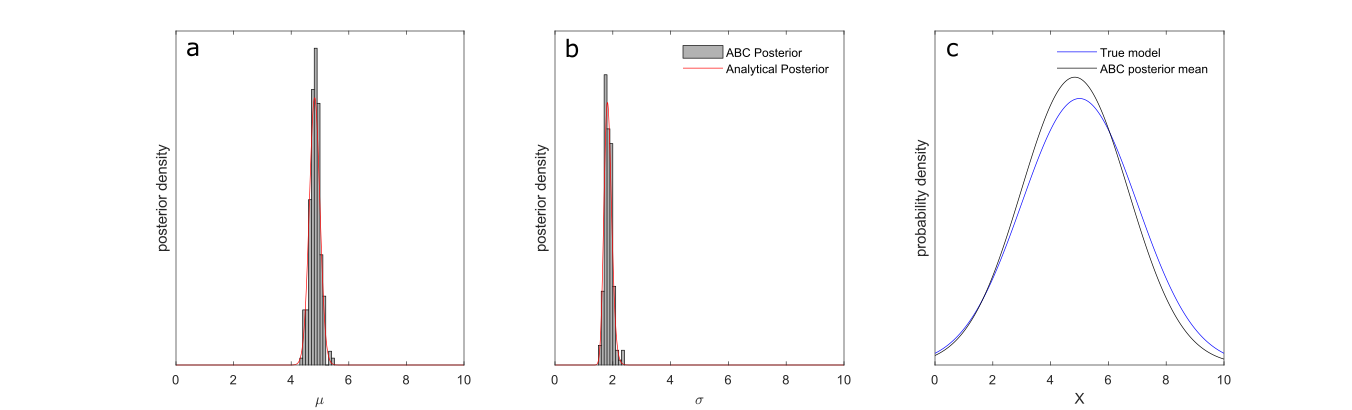
\includegraphics[scale=0.45]{toy1-fig1}
	\caption{Posterior comparison between ABC and traditional likelihood inference for estimating the parameters, $\bm{\theta} = [\mu,\sigma]$, to a Gaussian model given $n = 100$ observations, $\bm{y}$. The ABC algorithm, algorithm \ref{ABCrejectionsampler}, uses 1 million repititions and a tolerance $\epsilon = 0.1$. The likelihood takes the form $\mathcal{L}(\bm{\theta}|\bm{Y}) = (2\pi\sigma^2)^{-n/2}\ \text{exp}\big[-\frac{1}{2\sigma^2}\sum_{i = 1}^{n}(y_i-\mu)^2\big]$. (a) Marginal posterior compared to marginal ABC posterior for unknown parameter $\mu$. (b) same as (a) but for unknown parameter $\sigma$. (c) Mean ABC posterior model compared to true model.}
	\label{toy1-fig1}
\end{figure}

\begin{figure}[H]
	\centering
	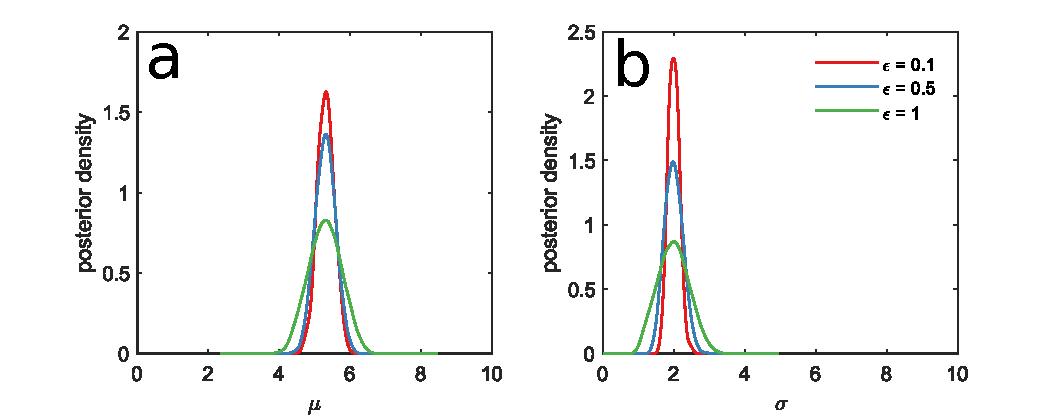
\includegraphics[scale=0.6]{toy1-fig2}
	\caption{The effect of varying the tolerance $\epsilon$ when estimating $\bm{\theta} = [\mu,\sigma]$ to a Gaussian model given given $n = 100$ observations, $\bm{y}$. Three tolerances are considered, $\epsilon = 0.1$, $\epsilon = 1$, $\epsilon = 5$. (a) Marginal ABC posterior for unknown parameter $\mu$. The true value is $\mu = 5$ (b) same as (a) but for unknown parameter $\sigma$. The true value is $\sigma = 2$}.
	\label{toy1-fig2}
\end{figure}

Figure \ref{toy1-fig1} demonstrates that with sufficient statistics and a low tolerance ABC can accurately resolve the posterior using only the ability to simulate data. However, as figure \ref{toy1-fig2} demonstrates, high tolerances significantly erode posterior accuracy and uncertainty is significantly over-estimated. However, it is true that increasing the tolerance increases the acceptance rate and hence relaxes computational resources. In this case the acceptance rate with $\epsilon = 0.1$ was $0.021\%$, while the acceptance rate with $\epsilon = 1$ was $2.023\%$. Under a model which is expensive to simulate from walking the tightrope between accuracy and efficiency becomes important and needs to be carefully examined. In spite of shortcomings, the strengths of the ABC rejection sampler has led to significant scientific experiments \citep{Fu1997,Weiss1998a,Pritchard1999a}.

\section{Toy problem 2: Linear regression}
As a second example consider we have observed some data, $\bm{y}$, from the linear model $\bm{g}(\bm{\theta}) = mx + b$ and there is some stochasticity in the measurement process such that $\bm{g_s}(\bm{\theta}) = \bm{g}(\bm{\theta}) + \mathcal{N}(0,\sigma^2)$. In total the unknown parameters constitute $\bm{\theta} = [m,b,\sigma]$. However, in this case it is deemed that computational resources are limitied and MCMC, which uses local transitions, will be needed to improve acceptance rates. MCMC will also be needed when the search spaces are high dimensional, many unknown parameters, and the posterior is a long way from the prior. For this case we can call upon ABC-MCMC in the form of algorithm \ref{ABC-MCMC}. \\

Algorithm \ref{ABC-MCMC} samples the ABC posterior, equation \ref{summary-stat-abc-posterior}. The algorithm relies on evaluating the M-H acceptance probability, equation \ref{M-H-acce}. In our implementations Gaussian transition kernels, $q(.,.)$, are strictly used. As such the transition kernels cancel out in equation \ref{M-H-acce}. That leaves the prior and the weighting kernel to be evalutated at each time step in the Markov chain. The weighting kernel takes the form of equation \ref{generic-weighting-kernel}. In this case a uniform weighting kernel, $K_U$, is implemented. The interpretation of $K_U$ is the same as the accept/reject step in the rejection sampler: 
\begin{equation}
	K_U = 1\ \text{if}\ \frac{|(S_i(\bm{y^*}) - S_i(\bm{y}))|}{\epsilon} \leq 1
\end{equation}
\begin{equation}
	K_U = 0\ \text{if}\ \frac{|(S_i(\bm{y^*}) - S_i(\bm{y}))|}{\epsilon} > 1
\end{equation}
$K_U$ hence forms an indicator function $\mathbbm{1}$ which is equal to $1$ when the distance between statistics, which are fit marginally, is less than the tolerance. Given, $\bm{S} = \{S_1,\dots,S_O\}$, the weighting kernel takes the form:
\begin{equation}
	p(\bm{S}(\bm{y})|\bm{S}(\bm{y^*}),\bm{\theta}) = \prod_{i = 1}^{O} K_U\Big(\frac{\rho(S_i(\bm{y}),S_i(\bm{y^*})}{\epsilon}\Big)
\end{equation}

As with the 1D Gaussian example it would be possible to take summaries which have a 1:1 correspondance to the unknown parameters. That is for a given simulation, a linear model could be fit to the simulated data and the slope and intercept of that fit used as summaries. However, to demonstrate that this is not necessary, we take inspiration from \citet{vrugt2013toward} and use mean, $\mu$, and standard deviation, $\sigma$, as summary statistics. The slope is restricted to a positive value to make these statistics sufficient. \\






\section{Toy problem 3: Bivariate Gaussian}




\section{Toy problem 4: Banana distribution}



 